\section{Casi d'uso}

\subsection{Attori dei casi d'uso}

\subsubsection{Attori primari}
\begin{figure}[H]
		\centering
		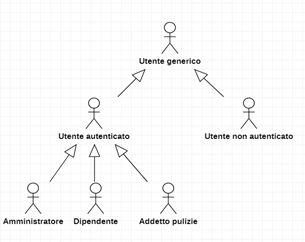
\includegraphics[width=10cm]{res/images/utentigenerali.png}
		\caption{Gerarchia degli attori principali}
		\label{fig:Gerarchia attori principali}
	\end{figure}

\textbf{Utente generico}\\
Si riferisce a un utente generico che accede alla piattaforma.\\
\\
\textbf{Utente non autenticato}\\
Si riferisce a un utente generico che non ha ancora effettuato l’autenticazione alla piattaforma.\\
\\
\textbf{Utente autenticato}\\
Si riferisce a un utente generico che si è autenticato nel sistema con la procedura di login.\\
\\
\textbf{Amministratore}\\
Si riferisce a un utente che si è autenticato nel sistema con il ruolo di amministratore.\\
\\
\textbf{Dipendente}\\
Si riferisce a un utente che si è autenticato nel sistema con il ruolo di dipendente.\\
\\
\textbf{Addetto pulizie}\\
Si riferisce a un utente che si è autenticato nel sistema con il ruolo di addetto alle pulizie.\\

\subsubsection{Attori secondari}
\textbf{Tag NFC}\\
Si riferisce ai tag presenti sulle postazioni. Ogni tag è assegnato a una postazione e permette di identificarla digitalmente.\\
\\
\textbf{Ethereum}\\
Si riferisce al servizio che memorizza su blockchain gli eventi di occupazione e igienizzazione delle postazioni.\\

\subsection{Elenco dei casi d'uso}
In questa sezione sono riportati tutti i casi d'uso individuati, ordinati per attore principale. Quando ritenuto utile, essi sono accompagnati da un grafico.
\\
\subsubsection{ UC1 - Guida introduttiva}
\begin{itemize}
           	\item\textbf{Attori Primari:} utente generico.
           	\item\textbf{Descrizione:} l'utente riceve una guida riguardo il login e il funzionamento.
           	\item\textbf{Scenario principale:} l’utente accede alla pagina introduttiva e visualizza la guida.
           	\item\textbf{Precondizione:} il sistema è raggiungibile e funzionante, l’utente accede alla pagina iniziale del sito della piattaforma.
           	\item\textbf{Postcondizione:} il sistema fornisce all’utente, attraverso la lettura della guida, tutte le istruzioni necessarie a effettuare il login.
\end{itemize}

\subsubsection{ UC2 - Login webserver}
\begin{itemize}
           	\item\textbf{Attori Primari:} utente non autenticato.
           	\item\textbf{Descrizione:} l’utente tenta di autenticarsi all'applicativo.
           	\item\textbf{Scenario principale:} l’utente non è ancora autenticato ed esegue il login inserendo nell'interfaccia del web server le seguenti credenziali:
           	\begin{itemize}
           		\item[$-$] nome utente;
           		\item[$-$] password.
           	\end{itemize}
           	\item\textbf{Estensioni:}
           	\begin{itemize}
           		\item[$-$] UC2.1 - Visualizzazione messaggio di errore;
           		\item[$-$] UC2.2 - Visualizzazione schermata relativa a utente non abilitato.
           	\end{itemize}
           	\item\textbf{Precondizione:} l’utente non si è autenticato nell'applicativo. 
           	\item\textbf{Postcondizione:} l’utente si è autenticato con successo ed è stato identificato dal sistema nel ruolo di amministratore, dipendente o addetto alle pulizie. A seconda della tipologia di utente vengono rese
           	disponibili diverse funzionalità.
\end{itemize}

\subsubsection{ UC2.1 - Visualizzazione messaggio di errore}
\begin{itemize}
	\item\textbf{Attori Primari:} utente non autenticato.
	\item\textbf{Descrizione:} l'utente visualizza un messaggio di errore dovuto al fatto che ha tentato il login ma ha sbagliato a inserire le credenziali.
	\item\textbf{Scenario principale:} l’utente tenta di eseguire la procedura di login all'applicativo.
	\item\textbf{Precondizione:} l'utente tenta di autenticarsi nell'applicativo.
	\item\textbf{Postcondizione:} viene visualizzato un messaggio di errore per informare l'utente del fatto che ha sbagliato a inserire le credenziali.
\end{itemize}
\subsubsection{ UC2.2 - Visualizzazione schermata relativa a utente non abilitato}
\begin{itemize}
	\item\textbf{Attori Primari:} utente non autenticato.
	\item\textbf{Descrizione:} l'utente tenta di autenticarsi nell'applicativo, tuttavia a causa della disabilitazione del suo account, il login viene interrotto, e
	l'utente visualizza il messaggio di errore che illustra la causa della disabilitazione dell'account.
	\item\textbf{Scenario principale:} l’utente non autenticato con account disabilitato tenta di autenticarsi. 
	La procedura di autenticazione viene bloccata a causa dello stato dell'account.
	\item\textbf{Precondizione:} un utente non autenticato, registrato all'applicativo e con account disabilitato tenta di effettuare il login automatico. 
	\item\textbf{Postcondizione:} viene visualizzato un messaggio di errore per informare l'utente del fatto che il 
	proprio account è stato disabilitato dall'amministratore. Se quest'ultimo, durante la procedura di disabilitazione, ha inserito un messaggio contenente la causa di tale azione, allora tale messaggio viene visualizzato.
\end{itemize}

\subsubsection{ UC3 - Login applicazione mobile}
\begin{itemize}
	\item\textbf{Attori Primari:} utente non autenticato.
	\item\textbf{Descrizione:} l’utente tenta di autenticarsi all'applicativo.
	\item\textbf{Scenario principale:} l’utente non è ancora autenticato ed esegue il login inserendo nell'interfaccia dell'applicazione mobile le seguenti credenziali:
	\begin{itemize}
		\item[$-$] nome utente;
		\item[$-$] password.
	\end{itemize}
	\item\textbf{Estensioni:}
	\begin{itemize}
		\item[$-$] UC3.1 - Visualizzazione messaggio di errore;
		\item[$-$] UC3.2 - Visualizzazione schermata relativa a utente non abilitato.
	\end{itemize}
	\item\textbf{Precondizione:} l’utente non si è autenticato nell'applicativo. 
	\item\textbf{Postcondizione:} l’utente si è autenticato con successo ed è stato identificato dal sistema
	nel ruolo di amministratore, dipendente o addetto alle pulizie. A seconda della tipologia di utente vengono rese
	disponibili diverse funzionalità.
\end{itemize}

\subsubsection{ UC3.1 - Visualizzazione messaggio di errore}
\begin{itemize}
	\item\textbf{Attori Primari:} utente non autenticato.
	\item\textbf{Descrizione:} l'utente visualizza un messaggio di errore dovuto al fatto che ha tentato il login ma ha sbagliato a inserire le credenziali.
	\item\textbf{Scenario principale:} l’utente tenta di eseguire la procedura di login all'applicativo.
	\item\textbf{Precondizione:} l'utente tenta di autenticarsi nell'applicativo.
	\item\textbf{Postcondizione:} viene visualizzato un messaggio di errore per informare l'utente del fatto che ha sbagliato a inserire le credenziali.
\end{itemize}
\subsubsection{ UC3.2 - Visualizzazione schermata relativa a utente non abilitato}
\begin{itemize}
           	\item\textbf{Attori Primari:} utente non autenticato.
           	\item\textbf{Descrizione:} l'utente tenta di autenticarsi nell'applicativo, tuttavia a causa della disabilitazione del suo account, il login viene interrotto, e
           	l'utente visualizza il messaggio di errore che illustra la causa della disabilitazione dell'account.
           	\item\textbf{Scenario principale:} l’utente non autenticato con account disabilitato tenta di autenticarsi. 
           	La procedura di autenticazione viene bloccata a causa dello stato dell'account.
           	\item\textbf{Precondizione:} un utente non autenticato, registrato all'applicativo e con account disabilitato tenta di effettuare il login automatico. 
           	\item\textbf{Postcondizione:} viene visualizzato un messaggio di errore per informare l'utente del fatto che il 
           	proprio account è stato disabilitato dall'amministratore. Se quest'ultimo, durante la procedura di disabilitazione, ha inserito un messaggio contenente la causa di tale azione, allora tale messaggio viene visualizzato.
\end{itemize}


\subsubsection{ UC4 - Logout amministratore}
\begin{itemize}
	\item\textbf{Attori Primari:} 
	amministratore.
	\item\textbf{Descrizione:} 
	l'amministratore si deautentica dal sistema.
	\item\textbf{Scenario principale:} 
	\begin{enumerate}
		\item l'utente autenticato preme un pulsante per la deautenticazione;
		\item l'utente viene deautenticato e portato alla schermata di login.
	\end{enumerate}
	\item\textbf{Precondizione:} 
	l'utente è autenticato nel sistema come amministratore.
	\item\textbf{Postcondizione:}
	l'utente non è autenticato nel sistema.
\end{itemize}

\subsubsection{ UC5 - Logout dipendente}
\begin{itemize}
	\item\textbf{Attori Primari:} 
	dipendente.
	\item\textbf{Descrizione:} 
	il dipendente si deautentica dal sistema.
	\item\textbf{Scenario principale:} 
	\begin{enumerate}
		\item l'utente autenticato preme un pulsante per la deautenticazione;
		\item l'utente viene deautenticato e portato alla schermata di login.
	\end{enumerate}
	\item\textbf{Precondizione:} 
	l'utente è autenticato nel sistema come dipendente.
	\item\textbf{Postcondizione:}
	l'utente non è autenticato nel sistema.
\end{itemize}

\subsubsection{ UC6 - Logout addetto alle pulizie}
\begin{itemize}
	\item\textbf{Attori Primari:} 
	addetto alle pulizie.
	\item\textbf{Descrizione:} 
	l'addetto alle pulizie si deautentica dal sistema.
	\item\textbf{Scenario principale:} 
	\begin{enumerate}
		\item l'utente autenticato preme un pulsante per la deautenticazione;
		\item l'utente viene deautenticato e portato alla schermata di login.
	\end{enumerate}
	\item\textbf{Precondizione:} 
	l'utente è autenticato nel sistema come addetto alle pulizie.
	\item\textbf{Postcondizione:}
	l'utente non è autenticato nel sistema.
\end{itemize}

\subsubsection{ UC7 - Guida amministratore}
\begin{itemize}
	\item\textbf{Attori Primari:} 
	amministratore.
	\item\textbf{Descrizione:} 
	l'amministratore ottiene una guida completa delle varie funzionalità.
	\item\textbf{Scenario principale:} 
	l'utente autenticato preme un pulsante per ottenere la guida completa.
	\item\textbf{Precondizione:} 
	l'utente è autenticato nel sistema come amministratore e vuole ottenere una guida.
	\item\textbf{Postcondizione:}
	l'utente può leggere la guida.
\end{itemize}

\subsubsection{ UC8 - Guida dipendente}
\begin{itemize}
	\item\textbf{Attori Primari:} 
	dipendente.
	\item\textbf{Descrizione:} 
	il dipendente ottiene una guida completa delle varie funzionalità.
	\item\textbf{Scenario principale:} 
	l'utente autenticato preme un pulsante per ottenere la guida completa.
	\item\textbf{Precondizione:} 
	l'utente è autenticato nel sistema come dipendente e vuole ottenere una guida.
	\item\textbf{Postcondizione:}
	l'utente può leggere la guida.
\end{itemize}

\subsubsection{ UC9 - Guida addetto alle pulizie}
\begin{itemize}
	\item\textbf{Attori Primari:} 
	addetto alle pulizie.
	\item\textbf{Descrizione:} 
	l'addetto alle pulizie ottiene una guida completa delle varie funzionalità.
	\item\textbf{Scenario principale:} 
	l'utente autenticato preme un pulsante per ottenere la guida completa.
	\item\textbf{Precondizione:} 
	l'utente è autenticato nel sistema come addetto alle pulizie e vuole ottenere una guida.
	\item\textbf{Postcondizione:}
	l'utente può leggere la guida.
\end{itemize}

\subsubsection{ UC10 - Visualizzazione stanze e postazioni}
\begin{figure}[H]
	\centering
	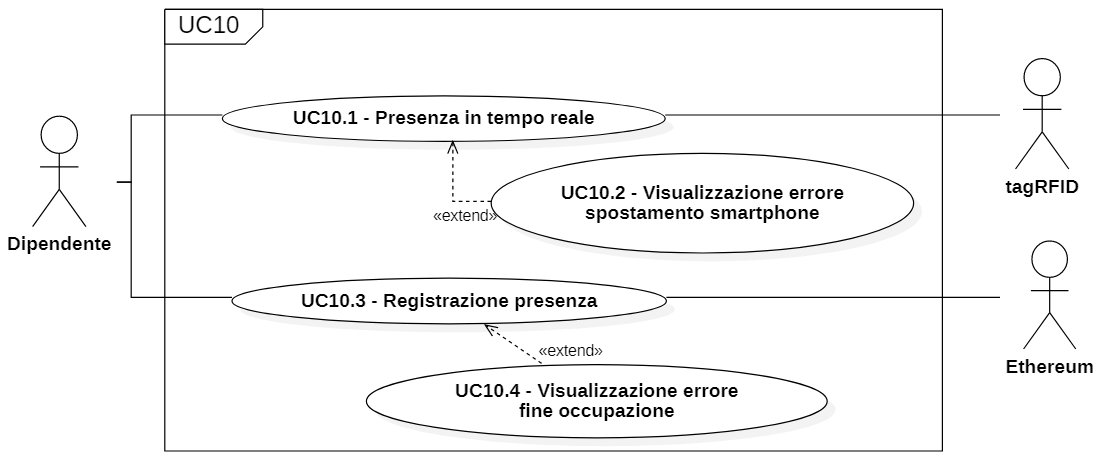
\includegraphics[width=15cm]{res/images/UC10.png}
	\caption{Stati postazioni}
	\label{fig:stati postazioni}
\end{figure}
\begin{itemize}
	\item\textbf{Attori Primari:}
	amministratore.
	\item\textbf{Descrizione:}
	il sistema mostra all'amministratore lo schema delle stanze e delle postazioni aggiornato rispetto alle azioni salvate su Ethereum.
	\item\textbf{Scenario principale:}
	\begin{enumerate}
		\item l'amministratore raggiunge la pagina di visione delle stanze e delle postazioni
		\item l'amministratore visualizza le stanze e le postazioni colorate in base al loro stato. Gli stati possibili sono:
		\begin{itemize}
			\item[$-$] libera e igienizzata;
			\item[$-$] libera e non igienizzata;
			\item[$-$] occupata;
			\item[$-$] prenotata e igienizzata;
			\item[$-$] prenotata e non igienizzata;
			\item[$-$] guasta e igienizzata;
			\item[$-$] guasta e non igienizzata.
		\end{itemize}
		Per ogni stanza è indicato il numero di occupanti attuali.
	\end{enumerate}
	\item\textbf{Precondizione:} 
	l'utente è autenticato come amministratore.
	\item\textbf{Postcondizione:}
	l'amministratore visualizza l'elenco delle stanze. Ogni stanza è rappresentata tramite una scacchiera. Ogni casella della scacchiera può indicare una postazione con il suo rispettivo stato e colore.
\end{itemize}


\subsubsection{ UC11 - Visualizzazione a calendario delle postazioni prenotate}
\begin{itemize}
	\item\textbf{Attori Primari:}
	amministratore.
	\item\textbf{Descrizione:}
	il sistema mostra all'amministratore un calendario con le prenotazioni delle postazioni.
	\item\textbf{Scenario principale:}
	l'utente raggiunge l'area di visualizzazione del calendario delle prenotazioni delle postazioni e lo visualizza.
	\item\textbf{Precondizione:} 
	l'utente è autenticato come amministratore.
	\item\textbf{Postcondizione:}
	l'amministratore visualizza il calendario delle prenotazioni delle postazioni.
\end{itemize}

\subsubsection{ UC12 - Creazione di una stanza}
\begin{itemize}
	\item\textbf{Attori Primari:}
	amministratore.
	\item\textbf{Attori Secondari:}
	Ethereum.
	\item\textbf{Descrizione:} 
	l'utente aggiunge una stanza al sistema.
	\item\textbf{Scenario principale:} 
	\begin{enumerate}
		\item l'utente autenticato preme un pulsante per creare una nuova stanza;
		\item compaiono i campi: "Nome della stanza" e "Dimensione della stanza" da compilare;
		\item l'utente compila i campi;
		\item l'utente preme un pulsante per confermare la creazione della stanza;
		\item se non è già presente una stanza con il codice inserito, essa viene creata;
		\item la configurazione della stanza viene inviata a Ethereum per essere salvata.
	\end{enumerate}
	\item\textbf{Estensione:}
	\begin{itemize}
		\item[$-$] UC12.1 - Avviso nome stanza già utilizzato
	\end{itemize}
	\item\textbf{Precondizione:} 
	l'utente è autenticato come amministratore.
	\item\textbf{Postcondizione:}
	è stata aggiunta una stanza vuota con le caratteristiche specificate.
\end{itemize}

\subsubsection{ UC12.1 - Avviso nome stanza già utilizzato}
\begin{itemize}
	\item\textbf{Attori Primari:}
	amministratore.
	\item\textbf{Descrizione:}
	l'utente tenta di assegnare alla stanza che sta creando un nome già utilizzato per un'altra stanza nel sistema e ne viene avvisato.
	\item\textbf{Scenario principale:}
	\begin{enumerate}
		\item l'utente inserisce come nome un valore già utilizzato;
		\item La stanza non viene creata e alla vista dell'utente compare un avviso che indica che il nome è già stato utilizzato. 
	\end{enumerate}
	\item\textbf{Precondizione:}
	l'utente si trova sulla pagina di creazione di una stanza.
	\item\textbf{Postcondizione:}
	l'utente visualizza il messaggio d'errore.
\end{itemize}

\subsubsection{ UC13 - Eliminazione di una stanza}
\begin{itemize}
	\item\textbf{Attori Primari:}
	amministratore.
	\item\textbf{Attori Secondari:}
	Ethereum.
	\item\textbf{Descrizione:} 
	l'utente elimina dal sistema una stanza con tutte le postazioni in essa presenti.
	\item\textbf{Scenario principale:} 
	\begin{enumerate}
		\item l'utente preme sul pulsante per l'eliminazione di una stanza;
		\item la stanza viene eliminata dal sistema con tutte le postazioni al suo interno;
		\item l'azione viene comunicata a Ethereum.
	\end{enumerate}
	\item\textbf{Precondizione:} 
	l'utente è autenticato.
	\item\textbf{Postcondizione:}
	è stata eliminata la stanza specificata, con tutte le postazioni al suo interno.
\end{itemize}

\subsubsection{UC14 - Modifica di una stanza}
\begin{itemize}
	\item\textbf{Attori Primari:}
	amministratore.
	\item\textbf{Attori Secondari:}
	Ethereum.
	\item\textbf{Descrizione:}
	l'utente modifica il codice identificativo di una stanza.
	\item\textbf{Scenario principale:} 
	\begin{enumerate}
		\item l'utente preme un pulsante per la modifica di una stanza;
		\item l'utente inserisce il nuovo nome;
		\item l'utente conferma il nuovo nome tramite un pulsante;
		\item se il nome non è già in utilizzo da parte di un'altra stanza, alla stanza selezionata viene assegnato il nome inserito;
		\item l'azione viene comunicata a Ethereum.
	\end{enumerate}
	\item\textbf{Estensioni:}
	\begin{itemize}
		\item[$-$] UC12.1 - Avviso nome stanza già utilizzato
	\end{itemize}
	\item\textbf{Precondizione:} 
	l'utente è autenticato.
	\item\textbf{Postcondizione:}
	il codice della stanza selezionata è stato modificato.
\end{itemize}

\subsubsection{UC15 - Impostazione di una stanza come inaccessibile.}
\begin{itemize}
	\item\textbf{Attori Primari:}
	amministratore.
	\item\textbf{Descrizione:}
	l'utente rende una stanza inaccessibile per alcuni giorni.
	\item\textbf{Scenario principale:} 
	\begin{enumerate}
		\item l'utente imposta: %il seguente elenco puntato è fatto così perchè se no mi dava errore%
			
				- data di inizio del periodo di inaccessibilità;
				
				- data di fine del periodo di inaccessibilità;
			
		\item l'utente conferma il periodo;
		\item l'inaccessibilità della stanza viene programmata per il periodo specificato.
	\end{enumerate}
	\item\textbf{Precondizione:} 
	l'utente è autenticato come amministratore e ha raggiunto l'area dedicata a questa azione.
	\item\textbf{Postcondizione:}
	l'inaccessibilità della stanza è stata programmata per le date specificate.
\end{itemize}

\subsubsection{UC16 - Creazione di una postazione}
\begin{itemize}
	\item\textbf{Attori Primari:}
	amministratore.
	\item\textbf{Attori Secondari:}
	Ethereum.
	\item\textbf{Descrizione:}
	l'amministratore crea una postazione e la assegna a una stanza.
	\item\textbf{Scenario principale:} 
	\begin{enumerate}
		\item l'amministratore preme un pulsante per aggiungere una nuova postazione;
		\item l'amministratore fornisce le seguenti informazioni:
		\begin{itemize}
			\item[$-$] codice della postazione;
			\item[$-$] codice del tag NFC che identifica la postazione;
			\item[$-$] posizione della postazione su una scacchiera rappresentante la stanza.
		\end{itemize}
		\item l'amministratore preme un bottone per la conferma dei dati;
		\item la postazione viene aggiunta all'interno della stanza;
		\item la nuova configurazione della stanza viene comunicata a Ethereum.
	\end{enumerate}
	\item\textbf{Estensioni:}
	\begin{itemize}
		\item[$-$] Avviso codice postazione già utilizzato (UC16.1);
		\item[$-$] Avviso codice tag già utilizzato (UC16.2);
		\item[$-$] Avviso posizione già occupata (UC16.3).
	\end{itemize}
	\item\textbf{Precondizione:} 
	l'utente è autenticato.
	\item\textbf{Postcondizione:}
	è stata inserita una nuova postazione all'interno di una stanza.
\end{itemize}

\subsubsection{UC16.1 - Avviso codice postazione già utilizzato}
\begin{itemize}
	\item\textbf{Attori Primari:}
	amministratore.
	\item\textbf{Descrizione:}
	l'utente tenta di assegnare a una postazione un codice già utilizzato attualmente per un'altra.
	\item\textbf{Scenario principale:}
	\begin{enumerate}
		\item l'utente sta creando o modificando una postazione e inserisce come codice un valore già utilizzato;
		\item la postazione non viene creata e alla vista dell'utente compare un avviso che indica che il codice è attualmente utilizzato.
	\end{enumerate}
	\item\textbf{Precondizione:}
	l'utente si trova sulla pagina di creazione o quella di modifica di una postazione.
	\item\textbf{Postcondizione:}
	l'utente visualizza il messaggio d'errore.
\end{itemize}

\subsubsection{UC16.2 - Avviso codice tag già utilizzato}
\begin{itemize}
	\item\textbf{Attori Primari:}
	amministratore.
	\item\textbf{Descrizione:}
	l'utente tenta di assegnare a una postazione il codice di un tag già utilizzato attualmente per un'altra.
	\item\textbf{Scenario principale:}
	\begin{enumerate}
		\item l'utente sta creando o modificando una postazione e inserisce come codice del tag corrispondente un valore già utilizzato;
		\item la postazione non viene creata e alla vista dell'utente compare un avviso che indica che il codice del tag è già assegnato a una postazione.
	\end{enumerate}
	\item\textbf{Precondizione:}
	l'utente si trova sulla pagina di creazione o quella di modifica di una postazione.
	\item\textbf{Postcondizione:}
	l'utente visualizza il messaggio d'errore.
\end{itemize}

\subsubsection{UC16.3 - Avviso posizione già occupata}
\begin{itemize}
	\item\textbf{Attori Primari:}
	amministratore.
	\item\textbf{Descrizione:}
	l'utente tenta di assegnare una posizione a una postazione già occupata.
	\item\textbf{Scenario principale:}
	\begin{enumerate}
		\item l'utente sta assegnando una posizione a una postazione, ma la posizione è già occupata;
		\item la postazione non viene creata e alla vista dell'utente compare un avviso che indica che la posizione è occupata.
	\end{enumerate}
	\item\textbf{Precondizione:}
	l'utente sta assegnando la posizione a una postazione.
	\item\textbf{Postcondizione:}
	l'utente visualizza il messaggio d'errore.
\end{itemize}

\subsubsection{UC17 - Eliminazione di una postazione}
\begin{itemize}
	\item\textbf{Attori Primari:}
	amministratore.
	\item\textbf{Attori Secondari:}
	Ethereum.
	\item\textbf{Descrizione:}
	l'utente elimina una postazione.
	\item\textbf{Scenario principale:} 
	\begin{enumerate}
		\item l'utente raggiunge l'area di eliminazione delle postazioni;
		\item l'utente preme un pulsante per l'eliminazione di una postazione;
		\item la postazione viene eliminata;
		\item la nuova configurazione della stanza viene inviata ad Ethereum.
	\end{enumerate}
	\item\textbf{Precondizione:} 
	l'utente è autenticato come amministratore.
	\item\textbf{Postcondizione:}
	una postazione è stata eliminata.
\end{itemize}

\subsubsection{ UC18 - Modifica di una postazione}
\begin{itemize}
	\item\textbf{Attori Primari:}
	amministratore.
	\item\textbf{Attori Secondari:}
	Ethereum.
	\item\textbf{Descrizione:}
	
	l'utente modifica gli attributi di una postazione.
	Gli attributi di una postazione sono:
	\begin{enumerate}
	\item codice della postazione;
	\item codice del tag NFC che identifica la postazione;
	\item posizione della postazione su una scacchiera rappresentante la stanza.
	\end{enumerate}
	
	\item\textbf{Scenario principale:} 
	\begin{enumerate}
		\item l'utente preme sul pulsante per la modifica di una postazione;
		\item inserisce i nuovi dati. Se la postazione non è occupata, è possibile impostarla come guasta. Se essa è già impostata come guasta, è possibile impostarla come libera. Lo stato di igienizzazione della postazione rimane invariato, come da diagramma degli stati di UC10;
		\item conferma i nuovi dati premendo un pulsante;
		\item i dati della postazione vengono modificati;
		\item il sistema invia i nuovi dati a Ethereum.
	\end{enumerate}
	\item\textbf{Estensioni:}
	\begin{itemize}
		\item[$-$] Avviso codice postazione già utilizzato (UC16.1);
		\item[$-$] Avviso codice tag già utilizzato (UC16.2);
		\item[$-$] Avviso posizione già occupata (UC16.3).
	\end{itemize}
	\item\textbf{Precondizione:} 
	l'utente è autenticato come amministratore.
	\item\textbf{Postcondizione:}
	sono stati aggiornati gli attributi della postazione selezionata.
\end{itemize}


\subsubsection{ UC19 - Visualizzazione lista credenziali}
\begin{figure}[H]
	\centering
	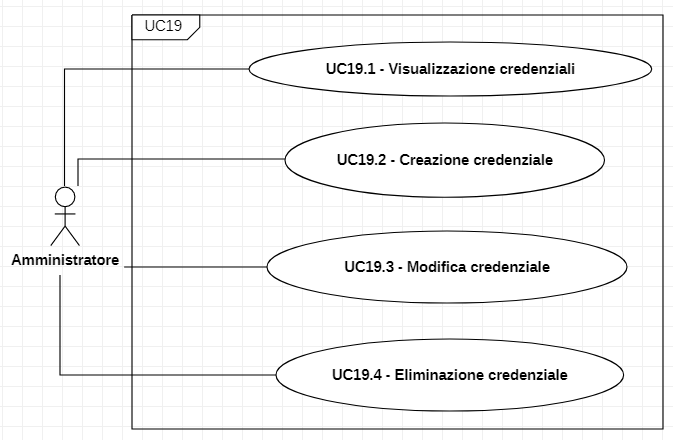
\includegraphics[width=18cm]{res/images/UC19.png}
	\caption{Visualizzazione lista credenziali}
	\label{fig:Visualizzazione lista credenziali}
\end{figure}
\begin{itemize}
	\item\textbf{Attori Primari:} 
	amministratore.
	\item\textbf{Descrizione:} 
	l'amministratore visualizza le credenziali di tutti gli utenti del sistema.
	\item\textbf{Scenario principale:} 
	l'utente naviga nell'interfaccia in modo da ottenere la visualizzazione delle credenziali.
	\item\textbf{Precondizione:} 
	l'utente è autenticato come amministratore.
	\item\textbf{Postcondizione:}
	l'utente visualizza la lista delle credenziali.
\end{itemize}

\subsubsection{ UC20 - Creazione di una credenziale}
\begin{figure}[H]
	\centering
	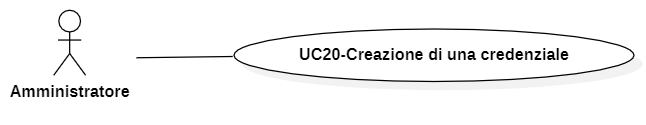
\includegraphics[width=18cm]{res/images/UC20.png}
	\caption{Creazione di una credenziale}
	\label{fig:Creazione di una credenziale}
\end{figure}
\begin{itemize}
	\item\textbf{Attori Primari:}
	amministratore.
	\item\textbf{Descrizione:} 
	l'amministratore crea una credenziale riservata a un qualsiasi utente del sistema: amministratore, dipendente o addetto alle pulizie.
	\item\textbf{Scenario principale:} 
	\begin{enumerate}
		\item l'amministratore naviga nell'interfaccia del sito web in modo da raggiungere l'ambiente di creazione delle credenziali;
		\item l'amministratore compila i seguenti campi:
		\begin{itemize}
			\item[$-$] nome;
			\item[$-$] cognome;
			\item[$-$] nome utente;
			\item[$-$] password;
			\item[$-$] e-mail.
		\end{itemize}
		Le credenziali vengono sempre create e abilitate. Questa proprietà può essere modificata successivamente, come descritto in UC21.
		\item l'amministratore preme il pulsante per la conferma dei dati;
		\item la nuova credenziale viene salvata nel sistema.
	\end{enumerate}
	\item\textbf{Precondizione:} 
	l'utente è autenticato come amministratore.
	\item\textbf{Postcondizione:}
	l'utente ha creato una nuova credenziale.
\end{itemize}

\subsubsection{ UC21 - Modifica di una credenziale}
\begin{figure}[H]
	\centering
	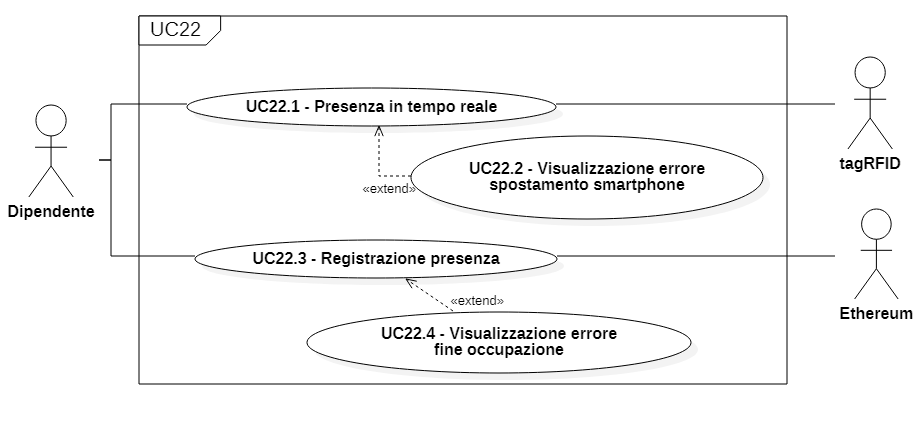
\includegraphics[width=18cm]{res/images/UC21.png}
	\caption{Modifica di una credenziale}
	\label{fig:Modifica di una credenziale}
\end{figure}
\begin{itemize}
	\item\textbf{Attori Primari:} 
	amministratore.
	\item\textbf{Descrizione:} 
	l'utente modifica i valori di un profilo utente.
	\item\textbf{Scenario principale:} 
	\begin{enumerate}
		\item l'amministratore naviga nell'interfaccia del sito web per accedere all'ambiente di modifica delle credenziali;
		\item l'amministratore inserisce i seguenti campi:
		\begin{itemize}
			\item[$-$] nome;
			\item[$-$] cognome;
			\item[$-$] nome utente;
			\item[$-$] password;
			\item[$-$] e-mail.
			\item[$-$] credenziali abilitate/disabilitate
		\end{itemize}		
		\item l'amministratore preme il pulsante per la conferma dei dati;
		\item i dati vengono aggiornati.
	\end{enumerate}
	\item\textbf{Precondizione:} 
	l'utente è autenticato come amministratore.
	\item\textbf{Postcondizione:}
	l'utente ha modificato un profilo utente.
\end{itemize}

\subsubsection{ UC22 - Eliminazione di una credenziale}
\begin{figure}[H]
	\centering
	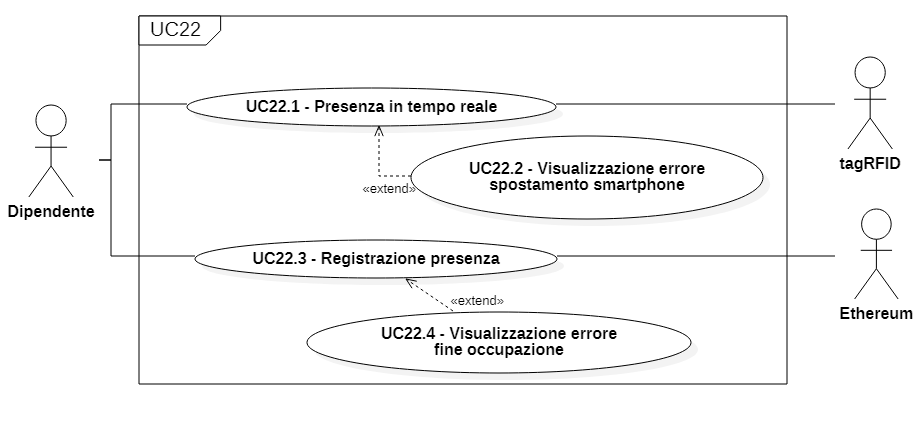
\includegraphics[width=18cm]{res/images/UC22.png}
	\caption{Eliminazione di una credenziale}
	\label{fig:Eliminazione di una credenziale}
\end{figure}
\begin{itemize}
	\item\textbf{Attori Primari:} 
	amministratore.
	\item\textbf{Descrizione:} 
	l'amministratore elimina delle credenziali dal sistema.
	\item\textbf{Scenario principale:} 
	\begin{enumerate}
		\item l'amministratore naviga nel sito web per raggiungere l'ambiente di eliminazione delle credenziali;
		\item l'amministratore preme sul pulsante per l'eliminazione delle credenziali;
		\item le credenziali selezionate sono eliminate dal sistema.
	\end{enumerate}
	\item\textbf{Precondizione:} 
	l'utente è autenticato come amministratore.
	\item\textbf{Postcondizione:}
	le credenziali selezionate non sono più presenti nel sistema.
\end{itemize}

\subsubsection{ UC23 - Esplorazione occupazioni delle postazioni}
\begin{figure}[H]
	\centering
	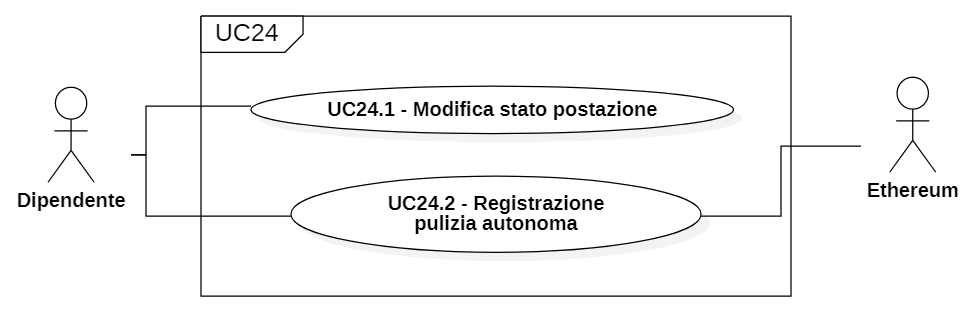
\includegraphics[width=18cm]{res/images/UC23.png}
	\caption{Esplorazione occupazioni delle postazioni}
	\label{fig:Esplorazione occupazioni delle postazioni}
\end{figure}
\begin{figure}[H]
	\centering
	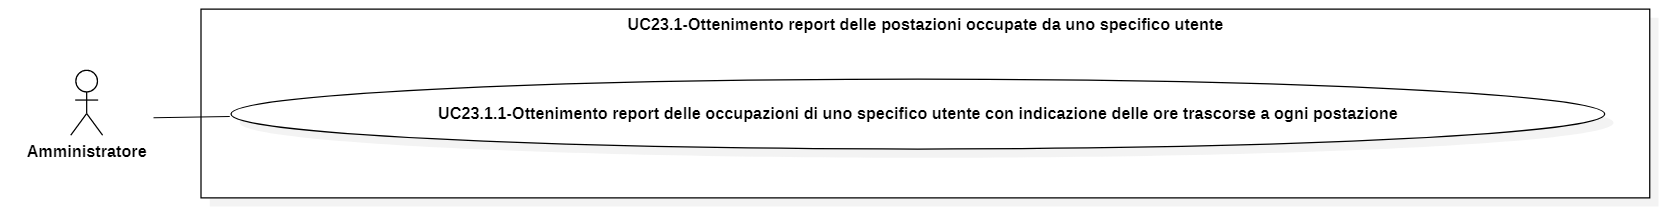
\includegraphics[width=18cm]{res/images/UC23.1.png}
	\caption{Ottenimento report delle postazioni occupate da uno specifico utente}
	\label{fig:Ottenimento report delle postazioni occupate da uno specifico utente}
\end{figure}
\begin{figure}[H]
	\centering
	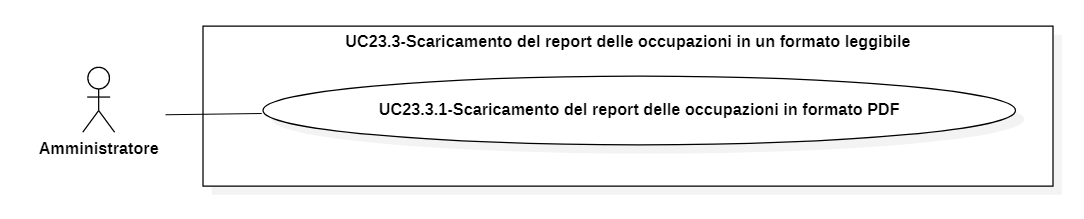
\includegraphics[width=18cm]{res/images/UC23.3.png}
	\caption{Scaricamento del report delle occupazioni in un formato leggibile}
	\label{fig:Scaricamento del report delle occupazioni in un formato leggibile}
\end{figure}
\begin{itemize}
	\item\textbf{Attori Primari:} 
	amministratore.
	\item\textbf{Descrizione:} 
	l'amministratore ottiene informazioni sugli eventi di occupazione, ovvero lo stato e da quali utenti sono occupate le postazioni.
	\item\textbf{Scenario principale:} 
	\begin{enumerate}
		\item l'amministratore raggiunge la pagina per la ricerca delle occupazioni delle postazioni;
		\item ricerca le informazioni a cui è interessato.
	\end{enumerate}	
	\item\textbf{Precondizione:} 
	l'utente è autenticato come amministratore.
	\item\textbf{Postcondizione:}
	l'utente visualizza le informazioni.
\end{itemize}

\subsubsection{ UC23.1 - Ottenimento report delle postazioni occupate da uno specifico utente}
\begin{itemize}
           	\item\textbf{Attori Primari:} 
           	amministratore.
           	\item\textbf{Descrizione:} 
           	l'amministratore ottiene informazioni in forma tabellare sulle postazioni occupate da uno specifico utente.
           	\item\textbf{Scenario principale:} 
           	\begin{enumerate}
           		\item l'utente inserisce il nome utente oppure il nome e cognome dell'utente a cui è interessato e il periodo all'interno del quale cercare, indicando date di inizio e di fine;
           		\item l'utente può opzionalmente specificare una postazione indicandone il codice;
           		\item nel report vengono visualizzate le date e ore di inizio e fine delle occupazioni e i codici delle postazioni.
           		Per ogni occupazione vengono visualizzati anche gli hash salvati sulla blockchain corrispondenti all'inizio e alla fine dell'occupazione e gli indirizzi in cui essi sono salvati.
           	\end{enumerate}
           	\item\textbf{Precondizione:} 
           	l'utente si trova sulla pagina per la ricerca delle occupazioni di uno specifico utente
           	\item\textbf{Postcondizione:}
           	l'utente visualizza le informazioni.
\end{itemize}


\subsubsection{ UC23.1.1 - Ottenimento report delle occupazioni di uno specifico utente con indicazione delle ore trascorse a ogni postazione}
\begin{itemize}
	\item\textbf{Attori Primari:} 
	amministratore.
	\item\textbf{Descrizione:} 
	l'amministratore ottiene informazioni in forma tabellare sulle postazioni occupate da uno specifico utente con l'indicazione delle ore trascorse in ogni postazione.
	\item\textbf{Scenario principale:}
	\begin{enumerate}
		\item l'ammistratore inserisce il nome utente oppure il nome e cognome dell'utente a cui è interessato e periodo all'interno del quale cercare, indicando date di inizio e di fine;
		\item l'utente può opzionalmente specificare una postazione indicandone il codice;
		\item nel report vengono visualizzate la data e ora di inizio e fine delle occupazioni, i codici delle postazioni e le ore trascorse;
		Per ogni occupazione vengono visualizzati anche gli hash salvati sulla blockchain corrispondenti all'inizio e alla fine dell'occupazione e gli indirizzi a cui essi sono salvati.
	\end{enumerate}
	\item\textbf{Precondizione:} 
	l'amministratore si trova sulla pagina per la ricerca delle occupazioni delle postazioni
	\item\textbf{Postcondizione:}
	l'utente visualizza le informazioni.
\end{itemize}

\subsubsection{ UC23.2 - Ottenimento report degli utenti che hanno occupato una specifica postazione}
\begin{itemize}
	\item\textbf{Attori Primari:} 
	amministratore.
	\item\textbf{Descrizione:} 
	l'amministratore ottiene informazioni in forma tabellare sulle occupazioni di una postazione.
	\item\textbf{Scenario principale:} 
	\begin{enumerate}
		\item l'amministratore inserisce il codice della postazione a cui è interessato e il periodo, indicando date di inizio e fine;
		\item l'utente può opzionalmente specificare un utente tramite nome utente oppure nome e cognome;
		\item nel report vengono visualizzate le date di inizio e fine delle occupazioni e i nomi degli utenti. Per ogni occupazione vengono visualizzati anche gli hash salvati sulla blockchain corrispondenti all'inizio e alla fine dell'occupazione e gli indirizzi a cui essi sono salvati.
	\end{enumerate}
	\item\textbf{Precondizione:} 
	l'amministratore si trova sulla pagina per la ricerca delle occupazioni delle postazioni
	\item\textbf{Postcondizione:}
	l'utente visualizza le informazioni specificate dalla sua ricerca.
\end{itemize}


\subsubsection{ UC23.3 - Scaricamento del report delle occupazioni in un formato leggibile}
\begin{itemize}
	\item\textbf{Attori Primari:} 
	amministratore.
	\item\textbf{Descrizione:} 
	l'amministratore scarica il report delle occupazioni che sta visualizzando in un formato leggibile.
	\item\textbf{Scenario principale:} 
	\begin{enumerate}
		\item l'amministratore preme un pulsante per lo scaricamento del report che sta visualizzando;
		\item il report viene scaricato.
	\end{enumerate}
	\item\textbf{Precondizione:} 
	l'utente sta visualizzando un report delle occupazioni, anche quello che indica i vicini di un utente(UC23.4 e UC23.4.1).
	\item\textbf{Postcondizione:}
	l'utente ha scaricato il report.
\end{itemize}

\subsubsection{ UC23.3.1 - Scaricamento del report delle occupazioni in formato PDF}
\begin{itemize}
	\item\textbf{Attori Primari:} 
	amministratore.
	\item\textbf{Descrizione:} 
	l'amministratore scarica il report delle occupazioni che sta visualizzando in formato \glock{PDF}.
	\item\textbf{Scenario principale:} 
	\begin{enumerate}
		\item l'amministratore preme un pulsante per lo scaricamento del report che sta visualizzando in formato PDF;
		\item il report viene scaricato in formato PDF.
	\end{enumerate}
	\item\textbf{Generalizzazione:}
	\begin{itemize}
		\item[$-$] scaricamento del report delle occupazioni in un formato leggibile (UC23.3).
	\end{itemize}
	\item\textbf{Precondizione:} 
	l'utente sta visualizzando un report.
	\item\textbf{Postcondizione:}
	l'utente ha scaricato il report in formato PDF.
\end{itemize}


\subsubsection{ UC23.4 - Report vicini utente}
\begin{itemize}
	\item\textbf{Attori Primari:} 
	amministratore.
	\item\textbf{Descrizione:} 
	l'amministratore ottiene un report dei vicini che l'utente selezionato ha avuto.
	\item\textbf{Scenario principale:} 
	\begin{enumerate}
		\item l'amministratore inserisce:
		\begin{itemize}
			\item[$-$] nome utente oppure nome e cognome del dipendente a cui è interessato;
			\item[$-$] data di inizio del periodo da considerare;
			\item[$-$] data di fine del periodo da considerare;
			\item[$-$] (opzionalmente) nome utente o nome e cognome di uno specifico utente da cercare tra i vicini.
		\end{itemize}
		\item l'amministratore riceve una lista degli utenti che hanno condiviso la stanza con l'utente selezionato. I vicini sono raggruppati per occupazione dell'utente selezionato: per ogni occupazione sono indicati gli utenti che in quel caso erano vicini a quello selezionato. Inoltre per ogni vicino sono indicate l'ora e la data di inizio e fine della vicinanza. Per ogni occupazione del dipendente e di ogni vicino sono indicati anche l'hash corrispondente e l'indirizzo sulla blockchain in cui l'hash è salvato.
	\end{enumerate}
	\item\textbf{Precondizione:} 
	l'amministratore si trova sulla pagina di esplorazione occupazioni.
	\item\textbf{Postcondizione:}
	l'amministratore visualizza un report di tutti i vicini che l'utente selezionato ha avuto nel periodo selezionato.
\end{itemize}


\subsubsection{ UC24 - Report igienizzazioni postazione}
\begin{itemize}
           	\item\textbf{Attori Primari:} 
           	amministratore.
           	\item\textbf{Descrizione:} 
           	l'amministratore ottiene una tabella delle igienizzazioni di tutte le postazioni con:
           	\begin{itemize}
           		\item[$-$] data e ora in cui sono avvenute;
           		\item[$-$] nome e cognome di chi le ha eseguite;
           		\item[$-$] ruolo di chi le ha eseguite (dipendente o addetto alle pulizie).
           	\end{itemize}
           	\item\textbf{Scenario principale:} 
           	l'amministratore visualizza la lista delle igienizzazioni con le informazioni correlate. Per ogni occupazione viene visualizzato anche l'hash salvato sulla blockchain corrispondente alla sanificazione e l'indirizzo in cui esso è salvato.
           	\item\textbf{Precondizione:} 
           	l'amministratore si trova sulla pagina di esplorazione delle igienizzazioni.
           	\item\textbf{Postcondizione:}
           	l'utente visualizza le informazioni.
\end{itemize}

\subsubsection{ UC24.1 - Scaricamento del report delle igienizzazioni in un formato leggibile}
\begin{itemize}
	\item\textbf{Attori Primari:} 
	amministratore.
	\item\textbf{Descrizione:} 
	l'amministratore scarica il report delle igienizzazioni che sta visualizzando in un formato leggibile.
	\item\textbf{Scenario principale:} 
	\begin{enumerate}
		\item l'amministratore preme un pulsante per lo scaricamento del report che sta visualizzando;
		\item il report viene scaricato.
	\end{enumerate}
	\item\textbf{Precondizione:} 
	l'utente sta visualizzando un report.
	\item\textbf{Postcondizione:}
	l'utente ha scaricato il report.
\end{itemize}

\subsubsection{ UC24.1.1 - Scaricamento del report delle igienizzazioni in formato PDF}
\begin{itemize}
	\item\textbf{Attori Primari:} 
	amministratore.
	\item\textbf{Descrizione:} 
	l'amministratore scarica il report delle igienizzazioni che sta visualizzando in formato PDF.
	\item\textbf{Scenario principale:} 
	\begin{enumerate}
		\item l'amministratore preme un pulsante per lo scaricamento del report che sta visualizzando in formato PDF;
		\item il report viene scaricato in formato PDF.
	\end{enumerate}
	\item\textbf{Generalizzazione:}
	\begin{itemize}
		\item[$-$] scaricamento del report delle igienizzazioni in un formato leggibile (UC24.1).
	\end{itemize}
	\item\textbf{Precondizione:} 
	l'utente sta visualizzando un report.
	\item\textbf{Postcondizione:}
	l'utente ha scaricato il report.
\end{itemize}



\subsubsection{ UC25 - Scansione tag NFC}
\begin{itemize}
	\item\textbf{Attori Primari:} dipendente.
	\item\textbf{Attori Secondari:} tag NFC.
	\item\textbf{Descrizione:} l’utente scansiona il tag NFC presente nella postazione per ricevere indicazioni sullo stato della stessa.
	\item\textbf{Scenario principale:} l’utente appoggia lo smartphone sul tag NFC.
	\item\textbf{Precondizione:} l’utente si è autenticato nell'applicazione mobile e attiva la funzionalità di scansione NFC.
	\item\textbf{Postcondizione:} l’utente ha effettuato correttamente la scansione.
\end{itemize}

\subsubsection{ UC26 - Visualizzazione stato postazione}
\begin{itemize}
	\item\textbf{Attori Primari:} dipendente.
	\item\textbf{Attori Secondari:} tag NFC.
	\item\textbf{Descrizione:} l’utente scansiona il tag NFC presente nella postazione per ricevere indicazioni sullo stato della stessa. I possibili stati sono:
	\begin{itemize}
		\item[$-$]libera e igienizzata;
		\item[$-$]libera e non igienizzata;
		\item[$-$]prenotata;
		\item[$-$]non accessibile.
	\end{itemize}
	Nel caso in cui una postazione risulti prenotata, viene mostrato il nome del dipendente che ha compiuto tale azione.
	\item\textbf{Scenario principale:} l’utente appoggia lo smartphone sul tag NFC e visualizza nell'applicazione mobile lo stato della postazione. 
	\item\textbf{Precondizione:} l’utente sta navigando nella sezione per la visualizzazione dello stato della postazione e 
	scansiona con il proprio smarthphone il tag NFC della postazione desiderata e visualizza il suo stato.
	\item\textbf{Postcondizione:} l’utente conosce lo stato della postazione ed eventualmente il nome del dipendente che ha effettuato la prenotazione della stessa.
\end{itemize}

\subsubsection{ UC27 - Segnalazione occupazione}
\begin{figure}[H]
	\centering
	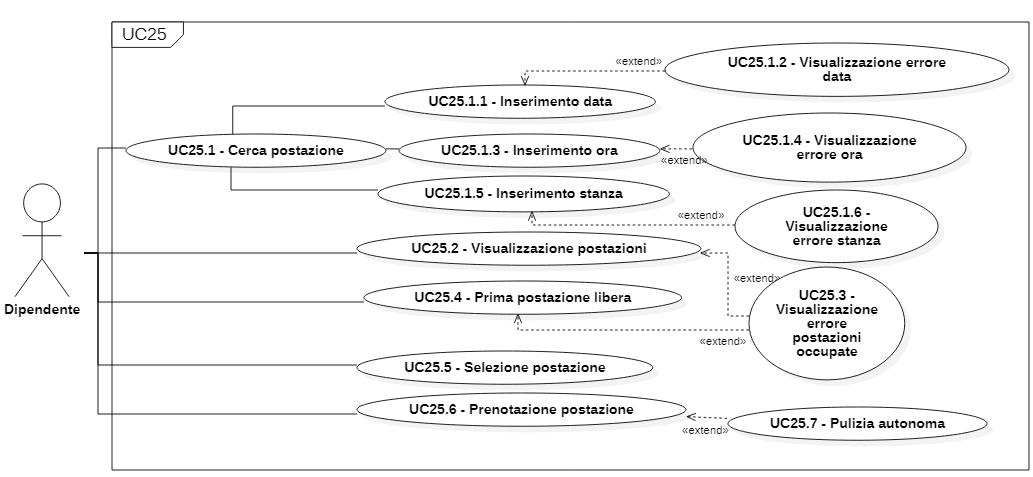
\includegraphics[width=15cm]{res/images/UC24.png}
	\caption{Segnalazione occupazione}
	\label{fig:Segnalazione occupazione}
\end{figure}
\begin{itemize}
	\item\textbf{Attori Primari:} dipendente.
	\item\textbf{Attori Secondari:} tag NFC, Ethereum.
	\item\textbf{Descrizione:} l’utente segnala in tempo reale la propria occupazione alla postazione, appoggiando lo smartphone sul tag NFC. Inoltre, registra il tempo di inizio e di fine di questa azione e lo comunica a Ethereum. Il primo è determinato da un timeout di un minuto in cui si lascia lo smartphone appoggiato sul tagNFC, mentre il secondo dal tempo di fine occupazione.
	\item\textbf{Scenario principale:} l’utente appoggia lo smartphone sul tag NFC e segnala in questo modo la propria occupazione.
	Il tempo di inizio e di fine di questa azione vengono memorizzati e comunicati a Ethereum.
	\item\textbf{Precondizione:} l’utente si è autenticato nell'applicazione mobile e occupa una postazione.
	\item\textbf{Postcondizione:} l’utente segnala in tempo reale l'occupazione alla postazione e registra questa azione su Ethereum.
\end{itemize}



\subsubsection{ UC27.1 - Occupazione in tempo reale}
\begin{itemize}
	\item\textbf{Attori Primari:} dipendente.
	\item\textbf{Attori Secondari:} tag NFC.
	\item\textbf{Descrizione:} l’utente segnala in tempo reale l'occupazione alla postazione, appoggiando lo smartphone sul tag NFC.
	\item\textbf{Scenario principale:} l’utente appoggia lo smartphone sul tag NFC e segnala in questo modo la propria occupazione in tempo reale.
	\item\textbf{Precondizione:} l’utente occupa una postazione e ha attivato nel proprio smartphone la possibilità di effettuare scansioni con tag NFC.
	\item\textbf{Postcondizione:} l’utente segnala in tempo reale l'occupazione alla postazione.
\end{itemize}


\subsubsection{ UC27.2 - Registrazione occupazione}
\begin{itemize}
	\item\textbf{Attori Primari:} dipendente.
	\item\textbf{Attori Secondari:} Ethereum.
	\item\textbf{Descrizione:} l’utente registra l'inizio e la fine della propria occupazione della postazione.
	\item\textbf{Scenario principale:} l'utente registra il tempo di inizio e di fine dell'occupazione di una postazione in modo automatico, grazie all'utilizzo di Ethereum. Il primo è determinato da un timeout di un minuto in cui si lascia lo smartphone appoggiato sul tagNFC, mentre il secondo dal tempo di fine occupazione.
	\item\textbf{Precondizione:} l’utente occupa una postazione e appoggia correttamente lo smartphone sul tag NFC. 
	\item\textbf{Postcondizione:} l'azione della precondizione viene registrata.
	\item\textbf{Estensioni:} 
	\begin{itemize}
		\item[$-$] visualizzazione errore fine prematura occupazione: se l'utente alza lo smartphone dal tag NFC e abbandona la postazione in modo prematuro rispetto al tempo di fine prenotazione, dopo mezzora viene visualizzato un messaggio di errore e avviene la disdetta automatica della prenotazione per il tempo rimanente (UC27.3);
	\end{itemize}
	\begin{itemize}
	\item[$-$] visualizzazione errore postazione non igienizzata: se la postazione non è pulita viene segnalato all'utente di igienizzarla (UC27.4).
	\end{itemize}
\end{itemize}

\subsubsection{ UC27.2.1 - Visualizzazione messaggio promemoria di inizio prenotazione}
\begin{itemize}
	\item\textbf{Attori Primari:} dipendente.
	\item\textbf{Descrizione:} l’utente visualizza un messaggio di inizio della prenotazione, 30 minuti prima che essa avvenga.
	\item\textbf{Scenario principale:} viene visualizzato un promemoria di inizio della prenotazione.
	\item\textbf{Precondizione:} l’utente ha effettuato una prenotazione almeno un'ora prima dell'inizio della stessa.
	\item\textbf{Postcondizione:} viene visualizzato un messaggio promemoria di inizio prenotazione della postazione.
\end{itemize}

\subsubsection{ UC27.2.2 - Visualizzazione messaggio promemoria di fine prenotazione}
\begin{itemize}
	\item\textbf{Attori Primari:} dipendente.
	\item\textbf{Descrizione:} l’utente visualizza un messaggio di fine della prenotazione, cinque minuti prima che essa avvenga.
	\item\textbf{Scenario principale:} viene visualizzato un promemoria di fine della prenotazione.
	\item\textbf{Precondizione:} l’utente ha effettuato una prenotazione.
	\item\textbf{Postcondizione:} viene visualizzato un messaggio promemoria di fine prenotazione della postazione.
\end{itemize}

\subsubsection{ UC27.3 - Visualizzazione fine prematura occupazione}
\begin{itemize}
	\item\textbf{Attori Primari:} dipendente.
	\item\textbf{Descrizione:} l’utente visualizza un messaggio in quanto sposta lo smartphone dal tag NFC, durante l'orario di prenotazione della postazione.
	\item\textbf{Scenario principale:} viene visualizzato un messaggio e avviene la disdetta automatica della prenotazione per il tempo restante.
	\item\textbf{Precondizione:} l’utente sposta il proprio smartphone dal tag NFC per un periodo di tempo maggiore o uguale a trenta minuti.
	\item\textbf{Postcondizione:} viene visualizzato un messaggio specifico e avviene la disdetta automatica della prenotazione per il tempo rimanente.
\end{itemize}

\subsubsection{ UC27.4 - Visualizzazione errore utente assente }
\begin{itemize}
	\item\textbf{Attori Primari:} dipendente.
	\item\textbf{Descrizione:} l'utente viene avvisato della disdetta automatica di una sua prenotazione.
	\item\textbf{Scenario Principale:} l'utente non ha ancora appoggiato il telefono sul tag NFC e sono passati trenta minuti dall'inizio della prenotazione:
	\begin{enumerate}
		\item la sua prenotazione viene disdetta;
		\item l'utente viene avvisato della disdetta tramite una notifica dell'applicazione.
	\end{enumerate}
	\item\textbf{Precondizione:} l'utente ha una prenotazione su una postazione.
	\item\textbf{Postcondizione:} viene visualizzato un messaggio di errore specifico e avviene la disdetta automatica della prenotazione per il tempo rimanente.
\end{itemize}

\subsubsection{ UC27.5 - Visualizzazione errore postazione non igienizzata}
\begin{itemize}
	\item\textbf{Attori Primari:} dipendente.
	\item\textbf{Descrizione:} l’utente visualizza un messaggio di errore in quanto non può occupare una postazione non igienizzata.
	\item\textbf{Precondizione:} l’utente appoggia il proprio cellulare sul tag NFC per segnalare l'occupazione. 
	\item\textbf{Postcondizione:} viene visualizzato un messaggio di errore specifico che avvisa finché la postazione non viene igienizzata non può essere occupata.
\end{itemize}



\subsubsection{ UC28 - Pulizia autonoma}
\begin{figure}[H]
	\centering
	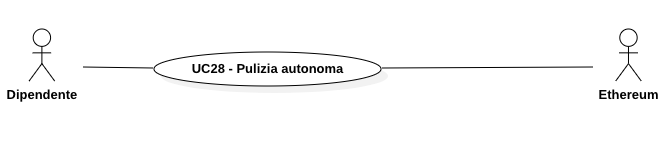
\includegraphics[width=18cm]{res/images/UC28_.png}
	\caption{Pulizia autonoma}
	\label{fig:Pulizia autonoma}
\end{figure}
\begin{itemize}
	\item\textbf{Attori Primari:} dipendente.
	\item\textbf{Attori Secondari:} Ethereum.
	\item\textbf{Descrizione:} l’utente pulisce in autonomia la postazione e lo segnala sull'applicazione mobile. Inoltre, 
	registra di aver effettuato questa azione, grazie all'utilizzo di Ethereum.	
	\item\textbf{Scenario principale:} l’utente segnala di aver igienizzato la postazione tramite l'applicazione mobile e automaticamente lo stato della postazione viene registrata come libera e igienizzata o prenotata e igienizzata. Inoltre, registra di aver effettuato questa azione, grazie all'utilizzo di Ethereum.
	\item\textbf{Precondizione:} l’utente è autenticato nell'applicazione mobile, ha igienizzato la propria postazione e sta navigando nella sezione per la pulizia 
	autonoma della postazione.
	\item\textbf{Postcondizione:} l’utente modifica lo stato della postazione in libera e igienizzata o prenotata e igienizzata e registra l'avvenuta pulizia autonoma della postazione.
\end{itemize}

\subsubsection{ UC29 - Cerca postazione}
\begin{figure}[H]
	\centering
	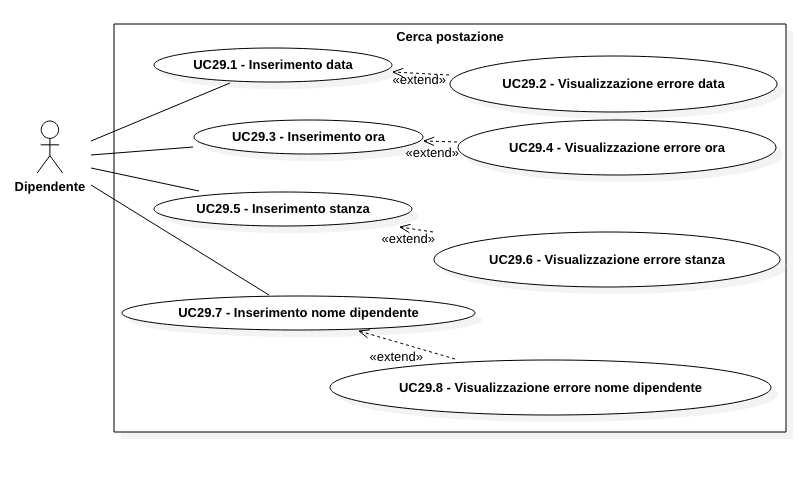
\includegraphics[width=18cm]{res/images/UC29.png}
	\caption{Cerca postazione}
	\label{fig:Cerca postazione}
\end{figure}
\begin{itemize}
	\item\textbf{Attori Primari:} dipendente.
	\item\textbf{Descrizione:} l’utente vuole prenotare una postazione di una stanza in un determinato giorno e orario.
	\item\textbf{Scenario principale:} 
	\begin{itemize}
		\item[$-$] l’utente inserisce la data (UC29.1);
		\item[$-$] l’utente inserisce l'orario (UC29.3);
		\item[$-$] l’utente inserisce l'identificativo della stanza (UC29.5);
		\item[$-$] l’utente inserisce in modo opzionale il nome e il cognome del collega a cui si vuole sedere vicino (UC29.7).
	\end{itemize}
	\item\textbf{Precondizione:} l’utente sta navigando nella sezione dell'applicazione dedicata alla ricerca di una postazione.
	\item\textbf{Postcondizione:} l’utente inserisce i campi necessari alla ricerca della postazione desiderata.
\end{itemize}
\subsubsection{ UC29.1 - Inserimento data }
\begin{itemize}
	\item\textbf{Attori Primari:} dipendente.
	\item\textbf{Descrizione:} l’utente sta cercando una postazione disponibile e deve compilare il campo della data.
	\item\textbf{Scenario principale:} l’utente ha compilato il campo data.
	\item\textbf{Precondizione:} l’utente sta compilando i campi richiesti per effettuare la ricerca.
	\item\textbf{Postcondizione:} l’utente ha compilato il campo richiesto.
	\item\textbf{Estensioni:} l’utente inserisce i campi necessari alla ricerca della postazione desiderata.
	\begin{itemize}
		\item[$-$] l’utente inserisce una data non valida (UC29.2).
	\end{itemize}
\end{itemize}
\subsubsection{ UC29.2 - Visualizzazione errore: data non valida  }
\begin{itemize}
	\item\textbf{Attori Primari:} dipendente.
	\item\textbf{Descrizione:} l’utente ha compilato un campo per la data, ma è in un formato non corretto.
	\item\textbf{Scenario principale:} 
	\begin{itemize}
		\item[$-$] l’utente ha inserito il campo per la data;
		\item[$-$] il sistema elabora la richiesta;
		\item[$-$] viene visualizzato un errore che segnala che la data non è valida.
	\end{itemize}
	\item\textbf{Precondizione:} l’utente ha compilato il campo per la data.
	\item\textbf{Postcondizione:} l'utente visualizza un messaggio di errore specifico e l'azione non viene portata a termine.
	\item\textbf{Estensioni:} l’utente inserisce i campi necessari alla ricerca della postazione desiderata.
	\begin{itemize}
		\item[$-$] l’utente inserisce un orario non valido (UC29.4).
	\end{itemize}
\end{itemize}
\subsubsection{ UC29.3 - Inserimento ora }
\begin{itemize}
	\item\textbf{Attori Primari:} dipendente.
	\item\textbf{Descrizione:} l’utente sta cercando una postazione disponibile e deve compilare il campo orario con granularità di un'ora.
	\item\textbf{Scenario principale:} l’utente ha compilato il campo orario.
	\item\textbf{Precondizione:} l’utente sta compilando i campi richiesti per effettuare la ricerca.
	\item\textbf{Postcondizione:} l’utente ha compilato il campo richiesto.
	\item\textbf{Estensioni:} l’utente inserisce i campi necessari alla ricerca della postazione desiderata.
	\begin{itemize}
		\item[$-$] l’utente inserisce una stanza non valida (UC29.6).
	\end{itemize}
\end{itemize}
\subsubsection{ UC29.4 - Visualizzazione errore: orario non valido }
\begin{itemize}
	\item\textbf{Attori Primari:} dipendente.
	\item\textbf{Descrizione:} l’utente ha compilato un campo per l'orario, ma è in un formato non corretto.
	\item\textbf{Scenario principale:} 
	\begin{itemize}
		\item[$-$] l’utente ha inserito il campo per l'orario;
		\item[$-$] il sistema elabora la richiesta;
		\item[$-$] viene visualizzato un errore che segnala che l'orario non è valido.
	\end{itemize}
	\item\textbf{Precondizione:} l’utente ha compilato il campo per l'orario.
	\item\textbf{Postcondizione:} l’utente visualizza un messaggio di errore specifico e non viene portata a termine l'azione.
\end{itemize}
\subsubsection{ UC29.5 - Inserimento stanza }
\begin{itemize}
	\item\textbf{Attori Primari:} dipendente.
	\item\textbf{Descrizione:} l’utente sta cercando una postazione disponibile e deve compilare il campo dell'identificativo della stanza.
	\item\textbf{Scenario principale:} l’utente ha compilato il campo dell'identificativo della stanza.
	\item\textbf{Precondizione:} l’utente sta compilando i campi richiesti per effettuare la ricerca.
	\item\textbf{Postcondizione:} l’utente ha compilato il campo richiesto.
\end{itemize}
\subsubsection{ UC29.6 - Visualizzazione errore: stanza non valida }
\begin{itemize}
	\item\textbf{Attori Primari:} dipendente.
	\item\textbf{Descrizione:} l’utente ha compilato un campo per l'identificativo della stanza, ma è in un formato non corretto.
	\item\textbf{Scenario principale:} 
	\begin{itemize}
		\item[$-$] l’utente ha inserito il campo per l'identificativo della stanza;
		\item[$-$] il sistema elabora la richiesta;
		\item[$-$] viene visualizzato un errore che segnala che l'identificativo della stanza non è valido.
	\end{itemize}
	\item\textbf{Precondizione:} l’utente ha compilato il campo per la stanza.
	\item\textbf{Postcondizione:} l’utente visualizza un messaggio di errore specifico e non viene portata a termine l'azione.
\end{itemize}

\subsubsection{ UC29.7 - Inserimento nome dipendente }
\begin{itemize}
	\item\textbf{Attori Primari:} dipendente.
	\item\textbf{Descrizione:} l’utente sta cercando una postazione disponibile e deve compilare il campo nome e cognome del dipendente a cui si vuole sedere vicino e che ha già effettuato una prenotazione.
	\item\textbf{Scenario principale:} l’utente ha compilato il campo nome e cognome.
	\item\textbf{Precondizione:} l’utente sta compilando il campo opzionale per effettuare la ricerca.
	\item\textbf{Postcondizione:} l’utente ha compilato il campo richiesto.
	\item\textbf{Estensioni:} l’utente inserisce i campi necessari alla ricerca della postazione desiderata.
	\begin{itemize}
		\item[$-$] l’utente inserisce un nome non valido (UC29.8).
	\end{itemize}
\end{itemize}
\subsubsection{ UC29.8 - Visualizzazione errore: nome dipendente non valido }
\begin{itemize}
	\item\textbf{Attori Primari:} dipendente.
	\item\textbf{Descrizione:} l’utente ha compilato un campo per il nome e il cognome del dipendente a cui si vuole sedere vicino, ma è in un formato non corretto.
	\item\textbf{Scenario principale:} 
	\begin{itemize}
		\item[$-$] l’utente ha inserito il campo per il nome e il cognome;
		\item[$-$] il sistema elabora la richiesta;
		\item[$-$] viene visualizzato un errore che segnala che  il nome e il cognome non sono validi.
	\end{itemize}
	\item\textbf{Precondizione:} l’utente ha compilato il campo per il nome e il cognome.
	\item\textbf{Postcondizione:} l’utente visualizza un messaggio di errore specifico e non viene portata a termine l'azione.
\end{itemize}
\subsubsection{ UC30 - Visualizzazione postazioni  }
\begin{figure}[H]
	\centering
	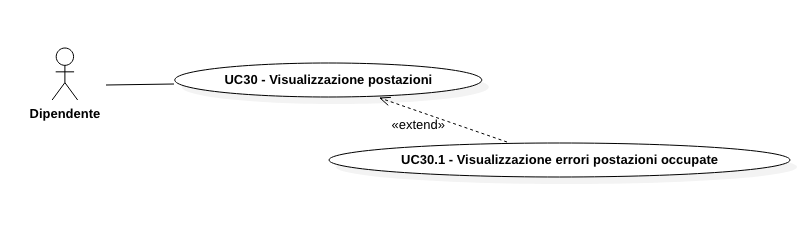
\includegraphics[width=18cm]{res/images/UC30.png}
	\caption{Visualizzazione postazioni }
	\label{fig:Visualizzazione postazioni }
\end{figure}
\begin{itemize}
	\item\textbf{Attori Primari:} dipendente.
	\item\textbf{Descrizione:} l’utente visualizza le postazioni con colori diversi in base allo stato. L'identificativo di una postazione è costituito da una lettera seguita da un numero (ad esempio: D10). 
	\item\textbf{Scenario principale:} viene visualizzato lo schema delle postazioni, rappresentato con colori diversi in base allo stato in cui si trovano.
	\item\textbf{Precondizione:} l’utente ha inserito i campi data, orario, stanza e in modo opzionale nome e cognome, correttamente e premuto il bottone di ricerca, nella sezione 
	medesima.
	\item\textbf{Postcondizione:} l’utente visualizza le postazioni nella stanza.
	\item\textbf{Estensioni:}
	\begin{itemize}
		\item[$-$] visualizzazione errore: tutte le postazioni nella stanza selezionata sono occupate o guaste (UC30.1).
	\end{itemize}
\end{itemize}
\subsubsection{ UC30.1 - Visualizzazione errore: postazioni occupate }
\begin{itemize}
	\item\textbf{Attori Primari:} dipendente.
	\item\textbf{Descrizione:} l’utente visualizza un messaggio di errore, in quanto non ci sono postazioni prenotabili.
	\item\textbf{Scenario principale:} 
	\begin{itemize}
		\item[$-$] l’utente ha inserito i campi data, orario, stanza;
		\item[$-$] il sistema elabora la richiesta;
		\item[$-$] viene visualizzato un messaggio di errore che consiglia di selezionare un'altra fascia oraria o stanza.
	\end{itemize}
	\item\textbf{Precondizione:} l’utente ha compilato i campi data, orario, stanza oppure ha selezionato la sezione prima postazione disponibile (UC31).
	\item\textbf{Postcondizione:} l’utente visualizza un messaggio di errore specifico e non viene portata a termine l'azione.
\end{itemize}
\subsubsection{ UC31 - Prima postazione libera }
\begin{figure}[H]
	\centering
	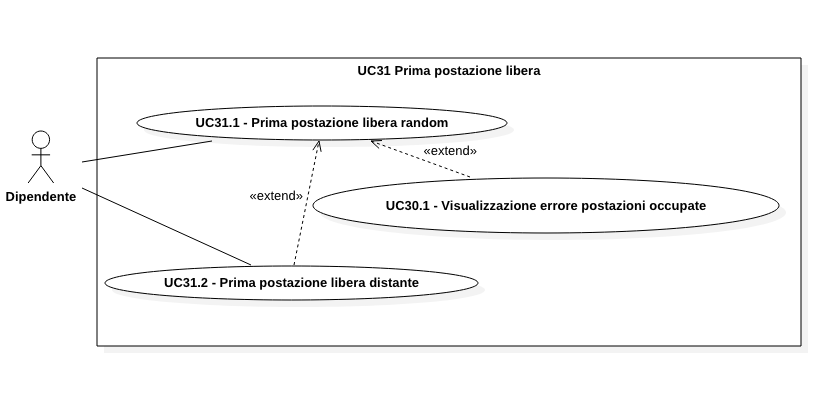
\includegraphics[width=18cm]{res/images/UC31.png}
	\caption{Prima postazione libera}
	\label{fig:Prima postazione libera}
\end{figure}
\begin{itemize}
	\item\textbf{Attori Primari:} dipendente.
	\item\textbf{Descrizione:} l’utente riceve l'identificativo di una postazione igienizzata e libera in una determinata stanza, 
	in modo automatico.
	\item\textbf{Scenario principale:} viene fornito l'identificativo di una postazione libera e igienizzata.
	\item\textbf{Precondizione:} l’utente preme il bottone nella sezione della prima postazione disponibile.
	\item\textbf{Postcondizione:} l’utente riceve l'identificativo di una postazione.
\end{itemize}
\subsubsection{ UC31.1 - Prima postazione libera random}
\begin{itemize}
	\item\textbf{Attori Primari:} dipendente.
	\item\textbf{Descrizione:} l’utente riceve l'identificativo di una postazione igienizzata e libera in una determinata stanza, 
	in modo automatico. La postazione proposta è libera per tutta la giornata lavorativa.
	\item\textbf{Scenario principale:} viene fornito l'identificativo di una postazione libera e igienizzata.
	\item\textbf{Precondizione:} l’utente preme il bottone nella sezione della prima postazione disponibile, libera per tutta la giornata lavorativa.
	\item\textbf{Postcondizione:} l’utente riceve l'identificativo di una postazione.
	\item\textbf{Estensioni:}
	\begin{itemize}
		\item[$-$] tutte le postazioni nella stanza selezionata sono occupate o guaste (UC30.1).
	\end{itemize}
\end{itemize}
\subsubsection{ UC31.2 - Prima postazione libera distante}
\begin{itemize}
	\item\textbf{Attori Primari:} dipendente.
	\item\textbf{Descrizione:} l’utente riceve l'identificativo di una postazione igienizzata e libera in una determinata stanza, 
	in modo automatico e in base a un criterio di distanziamento dalle altre postazioni.
	\item\textbf{Scenario principale:} viene fornito l'identificativo di una postazione libera e igienizzata.
	\item\textbf{Precondizione:} l’utente preme il bottone nella sezione della prima postazione disponibile, libera per tutta la giornata lavorativa e distanziata maggiormente dalle altre.
	\item\textbf{Postcondizione:} l’utente riceve l'identificativo di una postazione.
	\item\textbf{Estensioni:}
	\begin{itemize}
		\item[$-$] tutte le postazioni nella stanza selezionata sono occupate o guaste (UC30.1).
	\end{itemize}
\end{itemize}
\subsubsection{ UC32 - Prenotazione postazione }
\begin{figure}[H]
	\centering
	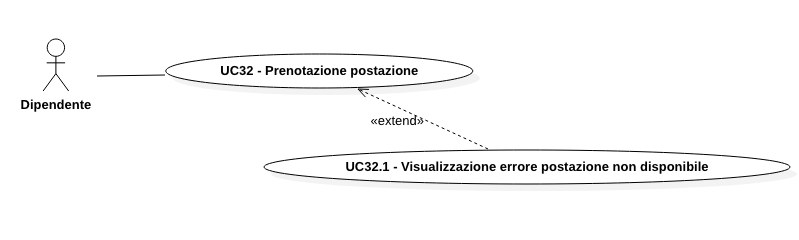
\includegraphics[width=18cm]{res/images/UC32.png}
	\caption{Prenotazione postazione}
	\label{fig:Prenotazione postazione}
\end{figure}
\begin{itemize}
	\item\textbf{Attori Primari:} dipendente.
	\item\textbf{Descrizione:} l’utente dopo aver selezionato la postazione, effettua la prenotazione. 
	\item\textbf{Scenario principale:} l’utente sta navigando nella sezione per la prenotazione di una postazione
	e preme il bottone per effettuare questa azione.
	\item\textbf{Precondizione:} l’utente ha selezionato correttamente la postazione di una stanza.
	\item\textbf{Postcondizione:} l'utente prenota la postazione.
	\item\textbf{Estensioni:}
	\begin{itemize}
		\item[$-$] nel caso in cui l'utente scelga di prenotare una postazione libera e igienizzata, ma ha già effettuato una prenotazione di un'altra postazione nella stessa data e orario (UC32.1).
	\end{itemize}
\end{itemize}
\subsubsection{ UC32.1 - Visualizzazione errore: postazione non prenotabile }
\begin{itemize}
	\item\textbf{Attori Primari:} dipendente.
	\item\textbf{Descrizione:} l’utente tenta di prenotare una postazione libera e igienizzata, ma ha già effettuato una prenotazione di una postazione nella stessa data e orario.
	\item\textbf{Scenario principale:} l'utente cerca di prenotare una postazione nonostante abbia già prenotato un'altra postazione in precedenza, nella stessa data e orario.
	\item\textbf{Precondizione:} l'utente prenota una postazione e nello stesso orario ne ha già un'altra.
	\item\textbf{Postcondizione:} l’utente visualizza un messaggio di errore specifico e non viene portata a termine l’azione.
\end{itemize}

\subsubsection{ UC33 - Prenotazione postazione automatica}
\begin{figure}[H]
		\centering
		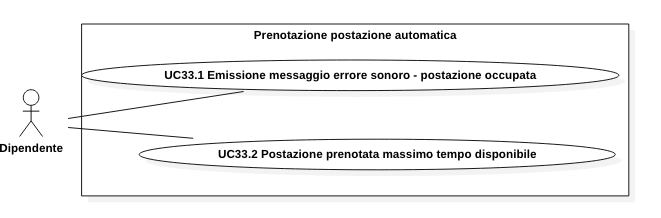
\includegraphics[width=18cm]{res/images/UC33.png}
		\caption{Prenotazione postazione automatica}
		\label{fig:Prenotazione postazione automatica}
	\end{figure}
\begin{itemize}
	\item\textbf{Attori Primari:} dipendente.
	\item\textbf{Descrizione:} l’utente dopo aver scansionato con il proprio smartphone il tag NFC per un tempo maggiore o uguale ad un minuto, prenota in modo automatico la postazione per l'intera giornata lavorativa. 
	\item\textbf{Scenario principale:} l’utente dopo aver scansionato con il proprio smartphone il tag NFC per un tempo maggiore o uguale ad un minuto, prenota in modo automatico la postazione per l'intera giornata lavorativa. Lo stato della postazione deve essere libera e igienizzata, e non prenotata durante il resto della giornata.
	\item\textbf{Precondizione:} l'utente lascia il telefono appoggiato al tag NFC di una postazione libera, più di un minuto.
	\item\textbf{Postcondizione:} l'utente prenota in modo automatico la postazione e inizia l'occupazione.
	\item\textbf{Estensioni:}
	\begin{itemize}
		\item[$-$] nel caso in cui l'utente scansiona per più di un minuto una postazione prenotata, viene emesso un segnale sonoro (UC33.1);
		\item[$-$] nel caso in cui l'utente scansiona per più di un minuto una postazione libera e igienizzata, ma prenotata in un determinato momento successivo della giornata, questa viene prenotata fino all'inizio della prenotazione successiva (UC33.2).
	\end{itemize}
\end{itemize}
\subsubsection{ UC33.1 - Emissione messaggio errore sonoro: postazione occupata}
\begin{itemize}
	\item\textbf{Attori Primari:} dipendente.
	\item\textbf{Descrizione:} l'utente sta scansionando per più di un minuto il tag NFC di una postazione prenotata, per cui viene emesso un segnale sonoro per farlo allontanare.
	\item\textbf{Scenario principale:} l’utente scansiona per più di un minuto il tag NFC di una postazione prenotata da un altro utente in precedenza.
	\item\textbf{Precondizione:} l'utente scansiona per più di un minuto una postazione prenotata.
	\item\textbf{Postcondizione:} viene emesso un segnale sonoro.
\end{itemize}

\subsubsection{ UC33.2 - Postazione prenotata massimo tempo disponibile}
\begin{itemize}
	\item\textbf{Attori Primari:} dipendente.
	\item\textbf{Descrizione:} l'utente sta scansionando per più di un minuto una postazione libera e igienizzata, ma prenotata in un determinato momento successivo della giornata. Quindi quest'ultima viene prenotata fino all'inizio della prenotazione successiva, che equivale al massimo tempo disponibile.
	\item\textbf{Scenario principale:} l'utente scansiona per più di un minuto il tag NFC di una postazione prenotata nelle ore successive.
	\item\textbf{Precondizione:} l'utente scansiona il tag NFC di una postazione prenotata nelle ore successive della giornata lavorativa.
	\item\textbf{Postcondizione:} l'utente prenota in modo automatico una postazione fino all'inizio della prenotazione successiva e inizia l'occupazione.
\end{itemize}

\subsubsection{ UC34 - Visualizzazione lista prenotazioni}
\begin{figure}[H]
		\centering
		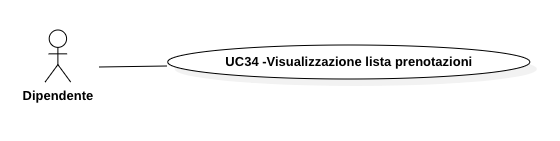
\includegraphics[width=18cm]{res/images/UC34.png}
		\caption{Visualizzazione lista prenotazioni}
		\label{fig:Visualizzazione lista prenotazioni}
	\end{figure}
\begin{itemize}
	\item\textbf{Attori Primari:} dipendente.
	\item\textbf{Descrizione:} l'utente visualizza la lista delle prenotazioni effettuate in precedenza. Ogni prenotazione contiene le seguenti informazioni:
	\begin{itemize}
		\item[$-$] orario di inizio prenotazione;
		\item[$-$] orario di fine prenotazione;
		\item[$-$] data;
		\item[$-$] identificativo postazione.
	\end{itemize}
	\item\textbf{Scenario principale:} l’utente visualizza la lista delle prenotazioni da lui effettuate.
	\item\textbf{Precondizione:} l'utente sta navigando nella sezione della lista delle prenotazioni effettuate.
	\item\textbf{Postcondizione:} l’utente visualizza le prenotazioni effettuate.
\end{itemize}

\subsubsection{ UC35 - Disdetta prenotazione}
\begin{figure}[H]
		\centering
		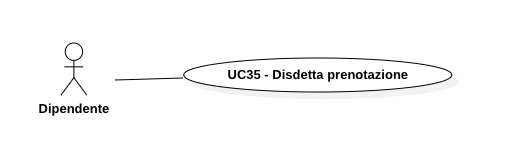
\includegraphics[width=18cm]{res/images/UC35.png}
		\caption{Disdetta prenotazione}
		\label{fig:Disdetta prenotazione}
	\end{figure}
\begin{itemize}
	\item\textbf{Attori Primari:} dipendente.
	\item\textbf{Descrizione:} l’utente disdice una prenotazione. 
	\item\textbf{Scenario principale:} l’utente disdice una prenotazione da lui effettuata in precedenza.
	\item\textbf{Precondizione:} l'utente sta navigando nella sezione della lista delle prenotazioni effettuate e ne ha selezionata una.
	\item\textbf{Postcondizione:} l’utente effettua la disdetta della prenotazione selezionata.
\end{itemize}

\subsubsection{ UC36 - Avviso indisponibilità postazione prenotata }
\begin{figure}[H]
		\centering
		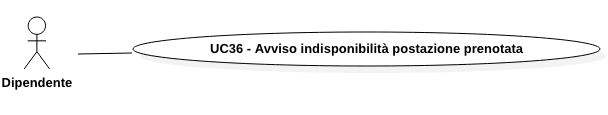
\includegraphics[width=18cm]{res/images/UC36.png}
		\caption{Avviso indisponibilità postazione prenotata}
		\label{fig:Avviso indisponibilità postazione prenotata}
	\end{figure}
\begin{itemize}
	\item\textbf{Attori Primari:} dipendente.
	\item\textbf{Descrizione:} il dipendente che ha una prenotazione per una postazione viene avvisato nel caso la postazione non sia più disponibile.
	\item\textbf{Scenario principale:} il dipente riceve una notifica che lo avvisa dell'indisponibilità di una postazione prenotata.
	\item\textbf{Precondizione:} l’utente è autenticato nell'applicazione mobile e ha almeno una postazione prenotata.
	\item\textbf{Postcondizione:} l'utente riceve una notifica che lo avvisa dell'indisponibilità di una delle postazioni che ha prenotato.
\end{itemize}

\subsubsection{UC37 - Elenco stanze da igienizzare}
\begin{figure}[H]
		\centering
		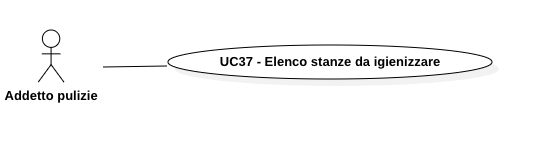
\includegraphics[width=18cm]{res/images/UC37.png}
		\caption{Elenco stanze da igienizzare}
		\label{fig:Elenco stanze da igienizzare}
	\end{figure}
\begin{itemize}
           	\item\textbf{Attori Primari:} addetto pulizie.
           	\item\textbf{Descrizione:} l'utente riceve un elenco delle stanze che necessitano di igienizzazione.
           	\item\textbf{Scenario principale:} l'utente si trova all'interno del sistema e verifica tutte le stanze che sono state utilizzate almeno da un dipendente, che saranno quindi da igienizzare.
           	\item\textbf{Precondizione:} l'utente va nella sezione dedicata nel sistema e deve premere un bottone.
           	\item\textbf{Postcondizione:} l'utente verifica quali stanze sono state occupate da almeno un dipendente, così da ottenere un elenco delle stanze da igienizzare.
\end{itemize}
\subsubsection{UC38 - Elenco postazioni da igienizzare}
\begin{figure}[H]
		\centering
		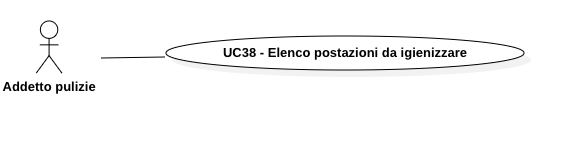
\includegraphics[width=18cm]{res/images/UC38.png}
		\caption{Elenco postazioni da igienizzare}
		\label{fig:Elenco postazioni da igienizzare}
	\end{figure}
\begin{itemize}
           	\item\textbf{Attori Primari:} addetto pulizie.
           	\item\textbf{Descrizione:} l'utente riceve un elenco delle postazioni che necessitano di igienizzazione.
           	\item\textbf{Scenario principale:} l'utente si trova all'interno del sistema e verifica tutte le postazioni che sono state utilizzate almeno da un dipendente, che saranno quindi da igienizzare.
           	\item\textbf{Precondizione:} l'utente va nella sezione dedicata nel sistema e deve premere un bottone.
           	\item\textbf{Postcondizione:} l'utente verifica quali postazioni sono state occupate da almeno un dipendente, così da ottenere un elenco delle postazioni da igienizzare.
\end{itemize}

\subsubsection{UC39 - Marcatura stanza come igienizzata}
\begin{figure}[H]
		\centering
		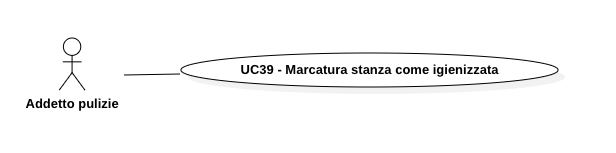
\includegraphics[width=18cm]{res/images/UC39.png}
		\caption{Marcatura stanza come igienizzata}
		\label{fig:Marcatura stanza come igienizzata}
	\end{figure}
\begin{itemize}
           	\item\textbf{Attori Primari:} addetto pulizie.
		\item\textbf{Attore Secondario:} Ethereum.
           	\item\textbf{Descrizione:} dopo l'igienizzazione l'utente marca la stanza come igienizzata.
           	\item\textbf{Scenario principale:} l'utente igienizza la stanza, in seguito accede al sistema e la marca come igienizzata attraverso l'utilizzo di Ethereum.
           	\item\textbf{Precondizione:} l'utente ottiene l'elenco delle stanze da igienizzare.
           	\item\textbf{Postcondizione:} l'utente, dopo l'igienizzazione, marca le stanze come igienizzate.
\end{itemize}
\subsubsection{UC40 - Marcatura postazione come igienizzata}
\begin{figure}[H]
		\centering
		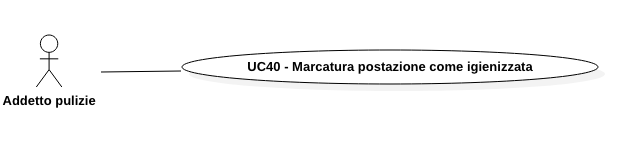
\includegraphics[width=18cm]{res/images/UC40.png}
		\caption{Marcatura postazione come igienizzata}
		\label{fig:Marcatura postazione come igienizzata}
	\end{figure}
\begin{itemize}
           	\item\textbf{Attori Primari:} addetto pulizie.
		\item\textbf{Attore Secondario:} Ethereum.
           	\item\textbf{Descrizione:} dopo l'igienizzazione l'utente marca la postazione come igienizzata.
           	\item\textbf{Scenario principale:} l'utente igienizza la postazione, in seguito accede al sistema e la marca come igienizzata attraverso l'utilizzo di Ethereum.
           	\item\textbf{Precondizione:} l'utente ottiene l'elenco delle postazioni da igienizzare.
           	\item\textbf{Postcondizione:} l'utente, dopo l'igienizzazione, marca le postazioni come igienizzate.
\end{itemize}
